\documentclass[10pt]{article}

% --- Faithful LaTeX conversion of docs/REPORT.md (M7). Content is verbatim: no number, CI,
% --- claim, citation, or caveat differs from the Markdown source. Compile from docs/:
% ---   cd docs && latexmk -pdf REPORT.tex      (or: pdflatex REPORT.tex twice; or: tectonic REPORT.tex)
\usepackage[utf8]{inputenc}
\usepackage[T1]{fontenc}
\usepackage[margin=0.9in]{geometry}
\usepackage{amsmath}
\usepackage{amssymb}
\usepackage{graphicx}
\usepackage{booktabs}
\usepackage{array}
\usepackage{caption}
\usepackage{microtype}
\usepackage{enumitem}
\usepackage[round]{natbib}
\usepackage[hidelinks]{hyperref}

\graphicspath{{../results/figures/}}

% Compact lists + tighter title/caption spacing to keep the report to 2--3 pages.
\setlist{itemsep=0pt, topsep=2pt, parsep=0pt}
\captionsetup{font=small, skip=4pt}
\setlength{\emergencystretch}{2em}  % absorb minor overfull boxes from long \texttt tokens

\title{Auditability, not accuracy: a head-to-head of Hybrid Confirmation\\
Trees and Learning-to-Defer on Galaxy Zoo}
\author{}
\date{June 2026}

\begin{document}
\maketitle
\vspace{-2.5em}

\section{Framing and contribution}

Human-AI decision pipelines are usually evaluated within a single family of methods: a
learning-to-defer (L2D) method against other L2D methods, or a confirmation rule against a
single-human or AI-alone baseline. In learning to defer, a policy routes some inputs to a human
instead of letting the model decide, trading the cost of querying a human for accuracy. The Hybrid
Confirmation Tree (HCT) of \citet{berger2026hct} (HCT-1; follow-up HCT-2,
\citealp{berger2026beyond}) and the L2D line of \citet{okati2021differentiable} and
\citet{MozannarS20} have, to our knowledge,
never been compared head-to-head on a shared dataset, backbone, and evaluation split. That
comparison is the contribution here. The Pareto plot is only its visualization. We adopt the
cost/accuracy trade-off framing of \citet{detoni2024predsets} (framing only; not implemented).

The result is a null: on the Galaxy Zoo binary task, with a shared strong AI backbone, no deployable
human-in-the-loop arm significantly beats AI-alone.

\section{Dataset and the non-expert-rater caveat}

HCT constrains the choice of dataset twice over. It is defined only for binary decisions, and it
needs real per-image multi-rater vote counts, on the order of 30 labels per image, to draw the two
simulated humans it consults. CIFAR-10H and ImageNet-16H are multiclass, so HCT is undefined on
them. HAM10000 ships no per-rater labels, so the
second human draw is impossible. Brinker's evaluation set of roughly 200 images has no statistical
power. Good Judgment Open is probabilistic forecasting with resolution lag, not instance-level
classification. Galaxy Zoo is the only candidate that is binary, carries 30+ real labels per image,
and ships with an original L2D author's code (Okati's), which removes one re-implementation. Once we
chosen, the same two constraints left no alternative.

We use the Galaxy Zoo binary 10k subset (spiral vs.\ early-type/smooth) that Okati 2021 uses (their
footnotes 8--9), sourced from the Kaggle Galaxy Zoo Challenge aggregate vote fractions. Each image
carries an urn of per-label vote counts over its 30+ raters. Drawing a simulated human means
sampling one label from that urn: HCT draws a first human $h_1$, and on disagreement a second $h_2$.
A drawn human is right or wrong about as often as a real volunteer. HCT
needs these real per-rater counts, which Okati's repository does not ship. The Kaggle competition
had anonymised its galaxy IDs, so the counts could not be looked up directly. We recover them by
matching each Kaggle galaxy's vote signature to the Willett et al.\ 2013 GZ2 catalog through a
content-based crosswalk: 5{,}904 of 10{,}000 images (59\%) match at high precision. After dropping
\texttt{star\_or\_artifact}-mode galaxies and images with too few votes for a without-replacement
draw, $N = 4{,}621$ survive (train 3{,}234 / val 693 / test 694). The matched subset is
morphologically representative (binary-hardness 0.52 vs.\ 0.48 overall), so the 41\% drop is not a
difficulty-selected bias. Coverage is 59\%, not the full set.

The raters are Galaxy Zoo citizen-science volunteers, not domain experts. Okati's ``human experts''
is loose terminology and this matters, since the single-human accuracy ceiling is the volunteer
crowd's, not an astronomer's. HCT's tie-breaking second draw $h_2$ comes from the same volunteer
vote distribution, so on genuinely ambiguous galaxies it is right only about as often as a coin
flip. Both effects depress the headroom available to any human-querying arm. The ``ground truth''
$y$ is itself the crowd-consensus majority, so every accuracy below is agreement with consensus, not
with objective truth (\S6).

\section{Methods and the invariants that make the comparison fair}

\begin{itemize}
  \item \textbf{AI-alone} --- the shared backbone thresholded at 0.5 (cost 0).
  \item \textbf{Single-human} --- one urn draw per image (cost 1).
  \item \textbf{HCT} (HCT-1, Fig.~1): the human $h_1$ and the binarized AI decide independently. If
    they agree, accept (cost 1). If they disagree, draw $h_2$ and take its call (cost 2). Expected
    human cost is $1 + P(\text{human--AI disagree})$, bounded in $[1,2]$, swept via the AI
    binarization threshold $\theta$, the only HCT knob. HCT is a decision rule, not a trained model.
  \item \textbf{L2D-Okati} (Thm.~3): for a fixed classifier, the optimal triage thresholds the
    per-instance gap between expected machine and human loss; a budget $b$ caps the deferral
    fraction. Cost is the deferral fraction $\in [0,1]$.
  \item \textbf{L2D-Mozannar} (eq.~10): the consistent convex surrogate $L_{\mathrm{CE}}^{\alpha}$;
    the deferral knob $\alpha$ sweeps a smooth curve. Cost is the deferral fraction $\in [0,1]$.
\end{itemize}

\paragraph{Shared-backbone and frozen-split invariants.}
Every arm consumes the same committed backbone scores and embeddings, and the same seed-0 70/15/15
split, guarded by a hash check. One shared metrics module computes all numbers.

\paragraph{Deviation: Option B.}
The L2D papers co-train classifier and rejector. We instead freeze the shared backbone and learn
only the rejector on top of its embeddings. This is because co-training would give each L2D arm
a different classifier, confounding the comparison with backbone differences. Freezing makes the AI
identical across all arms, so any measured gap is attributable to the deferral policy alone. It
removes a confound. The cost is that we measure these methods' triage quality, not their end-to-end
co-training, and we do not import their co-trained accuracy claims here.

\section{Results}

\begin{figure}[ht]
  \centering
  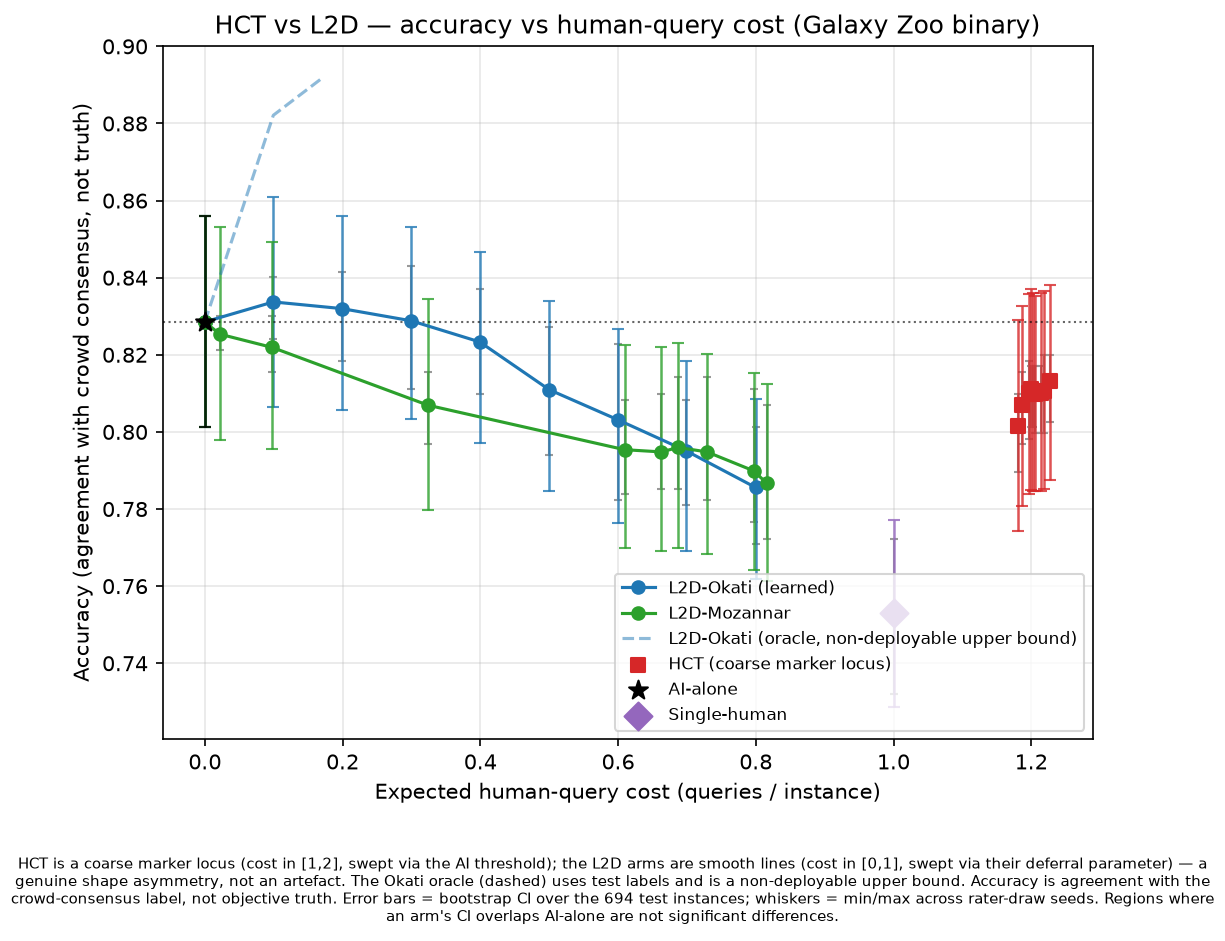
\includegraphics[width=0.52\linewidth]{pareto_frontier.png}
  \caption{HCT vs L2D: accuracy versus expected human-query cost on the Galaxy Zoo binary subset.}
  \label{fig:frontier}
\end{figure}

The horizontal axis, expected human-query cost, is the expected number of human labels queried per
decision: 0 for AI-alone, 1 for a single query, and up to 2 when HCT consults a second human. All
numbers come from the released results table. CIs are 95\% bootstrap over the 694 test instances,
with stochastic arms also resampled across rater-draw seeds [0--4]. The frontier is shown in
Figure~\ref{fig:frontier}.

\begin{table}[ht]
  \centering
  \small
  \begin{tabular}{@{}l c c p{4.2cm} c@{}}
    \toprule
    Arm (policy) & Accuracy [95\% CI] & Cost & vs AI-alone & Deployable \\
    \midrule
    \textbf{AI-alone} & \textbf{0.829 [0.801, 0.856]} & 0 & --- (baseline) & yes \\
    L2D-Okati (learned), $b{=}0.1$ & 0.834 [0.806, 0.861] & 0.10 & ns (CI overlaps) & yes \\
    L2D-Mozannar (best deferral, $\alpha{=}0.95$) & 0.822 [0.796, 0.849] & 0.10 & ns (CI overlaps), below mean & yes \\
    HCT ($\theta{=}0.1$) & 0.813 [0.788, 0.838] & 1.23 & ns (CI overlaps), below mean & yes \\
    Single-human & 0.753 [0.729, 0.777] & 1.00 & below (CI excludes 0.829) & yes \\
    L2D-Okati (\textbf{oracle}), $b{\approx}0.2$ & 0.892 [0.871, 0.911] & 0.17 & above, but non-deployable & no \\
    \bottomrule
  \end{tabular}
\end{table}

\paragraph{Curve-shape and cost-regime asymmetry.}
HCT is a coarse marker locus, drawn as discrete markers. Sweeping $\theta$ moves its expected cost
only within a narrow band, observed here as 1.18-1.23, because cost is $1 + P(\text{disagree})$ and
is structurally bounded in $[1,2]$. The L2D arms are smooth lines whose cost ranges over $[0,1]$.
The two methods therefore live in disjoint cost regimes, L2D in $[0,1]$ and HCT in $[1,2]$, and are
not mutually Pareto-comparable point for point. HCT is never drawn as a continuous curve. This is a
property of the methods, not of the plotting.

\paragraph{Reading the arms.}
L2D-Okati (learned) peaks at 0.834 at cost 0.10, then declines as more, often correct, machine
decisions are handed to noisier humans. Mozannar's best deferral point (0.822) sits below AI-alone
in the mean, though its CI still overlaps, and degrades further with deferral. HCT's accuracy is
flat at about 0.81 across $\theta$ and sits below AI-alone in the mean. The Okati oracle (dashed)
peeks at test labels to triage perfectly and climbs to 0.892, but it is a non-deployable upper bound
and is excluded from the deployable frontier.

\section{The central finding is an honest null}

No deployable arm significantly beats AI-alone. The verdict is computed mechanically in evaluation.
Every deployable arm's CI either overlaps AI-alone (L2D-Okati-learned, HCT, Mozannar) or sits
strictly below it. Single-human is the only arm whose CI excludes 0.829, and it is significantly
worse. L2D-Okati-learned's $+0.5$\,pt mean at cost 0.10 is within noise, and HCT's mean is below
AI-alone at cost above 1.

Interpretation: on consensus-labeled Galaxy Zoo with a strong AI, human deferral buys auditability,
not accuracy. HCT's value is that at least one human always approves the deployed decision, at a
bounded, transparent, training-free cost. That is a governance property, not an accuracy gain. The
oracle shows about 6 points of headroom exists in principle, but it is unrealizable with a
deployable rejector on these frozen embeddings, because the learned triage cannot identify which
machine errors a volunteer would fix.

\paragraph{Upstream self-claims are not findings here.}
HCT-1 \citep{berger2026hct} reports 28--44\% cost savings on its own datasets. That is a property of those datasets, not a
result on Galaxy Zoo, and we do not import it. Likewise we measure the L2D arms' triage over a
frozen backbone (Option B), not their co-trained end-to-end numbers. Every claim in this report
traces to a released artifact.

\section{Limitations}

\begin{itemize}
  \item \textbf{Single dataset, single backbone.} One task (Galaxy Zoo binary), one frozen
    ResNet-50. No claim generalizes beyond this setting.
  \item \textbf{Accuracy $=$ agreement with crowd consensus, not truth.} Because $y$ is the
    volunteer majority, a single human's accuracy is the majority vote share by construction, and
    HCT's $h_2$ is $\sim$50\% on near-split galaxies by construction. This compresses inter-arm gaps
    and is a threat to the comparison itself.
  \item \textbf{Non-expert raters} (\S2): the human ceiling and the $h_2$ tiebreak are
    volunteer-quality.
  \item \textbf{59\% crosswalk coverage} (\S2): 4{,}621 of 10{,}000; disclosed, representative, but
    not complete.
  \item \textbf{Urn structural limits.} $h_1 \perp h_2 \mid x$ is enforced, since both are
    independent draws from the same per-image distribution, so $h_2$ is a second \emph{draw}, not a
    second \emph{human}. The positive human--human correlation Berger studies lives only in
    between-image urn-composition variance, and the opinion-leader ($\rho$) reconstruction is not
    supported by aggregate counts.
  \item \textbf{Option-B deviation} (\S3): triage-only, not the papers' co-training; removes a
    backbone confound but does not evaluate end-to-end co-training.
  \item \textbf{Reproducibility.} The code and frozen artifacts needed to reproduce this report's
    figure and table are released\footnote{\url{https://github.com/Alessandro-vecchi/Rethinking-human-AI-decision-making}}, and regeneration is deterministic. The one-off backbone training
    and embedding export, and the raw-catalog label build sit upstream of that interface and are
    not re-run.
\end{itemize}

\bibliographystyle{plainnat}
\bibliography{references}

\end{document}
